\documentclass[12pt,a4paper,portrait]{article}
%\setcounter{secnumdepth}{0}
\usepackage{gensymb}
\usepackage{pdflscape}
\usepackage{amsmath}
\usepackage{amssymb}
\usepackage{enumitem}
\usepackage{graphicx}
\usepackage{subcaption}
\usepackage{multirow}
\usepackage{sansmath}
\setcounter{secnumdepth}{4}
\renewcommand\paragraph{\@startsection{paragraph}{4}{\z@}%
	% display heading, like subsubsection
	{-3.25ex\@plus -1ex \@minus -.2ex}%
	{1.5ex \@plus .2ex}%
	{\normalfont\normalsize\bfseries}\\}
\usepackage{pst-eucl}
\usepackage{multicol}
\usepackage{csquotes}
% Coding
\usepackage{listings}
\setlength{\parindent}{0pt}
\usepackage[obeyspaces]{url}
% Better inline directory listings
\usepackage{xcolor}
\definecolor{light-gray}{gray}{0.95}
\newcommand{\code}[1]{\colorbox{light-gray}{\texttt{#1}}}
\usepackage{adjustbox}
\usepackage[UKenglish]{isodate}
\usepackage[UKenglish]{babel}
\usepackage{float}
\usepackage[T1]{fontenc}
\usepackage{setspace}
\usepackage{sectsty}
\usepackage{longtable}
\newenvironment{tightcenter}{%
	\setlength\topsep{0pt}
	\setlength\parskip{0pt}
	\begin{center}
	}{%
	\end{center}
}
\captionsetup{width=\textwidth}
\usepackage{mbenotes} % to print table notes!
\usepackage{alphalph} % For extended counters!
% usage: \tabnotemark[3]\cmsp\tabnotemark[4]
\usepackage[colorlinks=true,linkcolor=blue,urlcolor=black,bookmarksopen=true]{hyperref}
\sectionfont{%			            % Change font of \section command
	\usefont{OT1}{phv}{b}{n}%		% bch-b-n: CharterBT-Bold font
	\sectionrule{0pt}{0pt}{-5pt}{3pt}}
\subsectionfont{
	\usefont{OT1}{phv}{b}{n}}
\newcommand{\MyName}[1]{ % Name
	\usefont{OT1}{phv}{b}{n} \begin{center}of {\LARGE  #1}\end{center}
	\par \normalsize \normalfont}
\makeatletter
\newcommand\FirstWord[1]{\@firstword#1 \@nil}%
\newcommand\@firstword{}%
\newcommand\@removecomma{}%
\def\@firstword#1 #2\@nil{\@removecomma#1,\@nil}%
\def\@removecomma#1,#2\@nil{#1}
\makeatother

\newcommand{\MyTitle}[1]{ % Name
	\Huge \usefont{OT1}{phv}{b}{n} \begin{center}#1\end{center}
	\par \normalsize \normalfont}
\newcommand{\NewPart}[1]{\section*{\uppercase{#1}}}
\newcommand{\NewSubPart}[1]{\subsection*{\hspace{0.2cm}#1}}
\renewcommand{\baselinestretch}{1.05}
\usepackage[margin=0.2cm]{geometry}
\date{}
\setcounter{tocdepth}{4}

\title{Double pendulum: damping and non-zero mass of bobs and rods}
\author{Brenton Horne}

\begin{document}
	\maketitle
	\tableofcontents
	
	\section{Introduction}
	The problem of the double pendulum has been widely analysed in the mechanics literature. Its most simplified version involves two pendulums, with the second attached to the first at the bob, the rods being massless and there being no friction and air resistance. Even this simplified version is subject to chaos and has equations of motion far more complicated than that of the simple pendulum.  
	\begin{figure}[H]
		\centering
		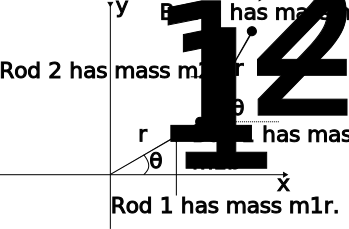
\includegraphics[width=300px]{Double pendulum.png}
		\caption{Diagram of a double pendulum with important components and variables labelled.}
	\end{figure}
	Figure 1 depicts the double pendulum system being analysed. Most physicists treat $\theta_1$ and $\theta_2$ as being relative to the negative y-axis instead of the positive x-axis. I, as primarily a mathematician, prefer the positive x-axis as the point of reference for angles as I find it more intuitive. 
	
	\section{Euler-Lagrange equations with generalized dissipation force}
	To obtain our equations of motion, we must apply the Euler-Lagrange equations with generalized dissipation force ($Q_i$ which is on the right-hand side of the following equation)
	
	\begin{align}
		\dfrac{d}{dt}\dfrac{\partial \mathcal{L}}{\partial \dot{q_i}} - \dfrac{\partial \mathcal{L}}{\partial q_i} &=  \sum_j \vec{F}_{D,j} \cdot \dfrac{\partial \vec{r}_j}{\partial q_i}. \label{ELD}
	\end{align}
	
	Where
	\begin{itemize}
		\item $\mathcal{L}$ is the Lagrangian --- the difference between the kinetc energy and potential energy of the system. 
		\item $(q_i)=(\theta_1,\theta_2)$ are the generalized coordinates of the system.
		\item $j=1b,1r,2b,2r$ refers to the moving components of our double pendulum system, namely the two bobs and two rods.
		\item $\vec{F}_{D,j}$ is the dissipation forces acting on the $j$th component of the system.
		\item $\vec{r}_j$ is the position vector for the $j$th component of the system.
		\item $\vec{e}_{j,i}=\dfrac{\partial \vec{r}_j}{\partial q_i}$ is the generalized basis vector.
	\end{itemize}
	
	
	\section{Position, velocity and generalized basis vector}
	\subsection{Bob 1}
	The first pendulum bob would have the coordinates, velocity and generalized basis vector
	\begin{align*}
		x_{1b} &= r_1 \cos{\theta_1} &\implies \dot{x}_{1b} &= -r_1\dot{\theta}_1 \sin{\theta_1}\\
		y_{1b} &= r_1 \sin{\theta_1} &\implies \dot{y}_{1b} &= r_1 \dot{\theta}_1 \cos{\theta_1} \\
		\vec{r}_{1b} &= \begin{bmatrix}
			x_{1b}\\
			y_{1b}
		\end{bmatrix}  &\therefore \vec{v}_{1b} &= \dfrac{d \vec{r}_{1b}}{dt}\\
		&= r_1\begin{bmatrix}
				-\sin{\theta_1} \\
				\cos{\theta_1}
			\end{bmatrix} & &=r_1\dot{\theta}_1 \begin{bmatrix}
			-\sin{\theta_1} \\
			\cos{\theta_1}
		\end{bmatrix} \\
		\vec{e}_{1b,\theta_1} &= \dfrac{\partial \vec{r}_{1b}}{\partial \theta_1}& v_{1b}^2 &= \dot{x}_{1b}^2 + \dot{y}_{1b}^2 \\
		&= r_1 \begin{bmatrix}
			-\sin{\theta_1}\\
			\cos{\theta_1}
		\end{bmatrix} & &= \left(-r_1\dot{\theta}_1 \sin{\theta_1}\right)^2 + \left(r_1 \dot{\theta}_1 \cos{\theta_1}\right)^2 \\
		\vec{e}_{1b,\theta_2} &= \dfrac{\partial \vec{r}_{1b}}{\partial \theta_2} &&= r_1^2 \dot{\theta}_1^2\\
		&= \begin{bmatrix}
			0\\
			0
		\end{bmatrix}.
	\end{align*}
	
	\subsection{Rod 1}
	The first pendulum rod would have the coordinates, velocity and generalized basis vector below. It is important to note that we are analysing its effect on the motion of the pendulum based on the centre of mass approach. 
	\begin{align*}
		x_{1r} &= \dfrac{r_1\cos{\theta_1}}{2} &\implies \dot{x}_{1r} &= -\dfrac{r_1\dot{\theta}_1\sin{\theta_1}}{2}\\
		y_{1r} &= \dfrac{r_1\sin{\theta_1}}{2} &\implies \dot{y}_{1r} &= \dfrac{r_1\dot{\theta}_1\cos{\theta_1}}{2}\\
		\vec{r}_{1r} &= \begin{bmatrix}
			x_{1r} \\
			y_{1r}
		\end{bmatrix} &\therefore \vec{v}_{1r} &= \dfrac{d\vec{r}_{1r}}{dt} \\
		&= \dfrac{r_1}{2}\begin{bmatrix}
			\cos{\theta_1}\\
			\sin{\theta_1}
		\end{bmatrix} & &= \dfrac{r_1\dot{\theta}_1}{2} \begin{bmatrix}
			-\sin{\theta_1}\\
			\cos{\theta_1}
		\end{bmatrix} \\
		\vec{e}_{1r,\theta_1} &= \dfrac{\partial \vec{r}_{1r}}{\partial \theta_1} & v_{1r}^2 &= \dot{x}_{1r}^2 + \dot{y}_{1r}^2 \\
		&= \dfrac{r_1}{2} \begin{bmatrix}
			-\sin{\theta_1}\\
			\cos{\theta_1}
		\end{bmatrix} & &= \left(-\dfrac{r_1\dot{\theta}_1 \sin{\theta_1}}{2}\right)^2 + \left(\dfrac{r_1 \dot{\theta}_1 \cos{\theta_1}}{2}\right)^2 \\
	\vec{e}_{1r,\theta_2} &= \dfrac{\partial \vec{r}_{1r}}{\partial \theta_2} &&= \dfrac{r_1^2 \dot{\theta}_1^2}{4} \\
	&= \begin{bmatrix}
		0 \\
		0
	\end{bmatrix}.
	\end{align*}
	
	\subsection{Bob 2}
	\begin{align*}
		x_{2b} &= x_{1b} + r_2 \cos{\theta_2} &\dot{x}_{2b} &= -r_1\dot{\theta}_1 \sin{\theta_1}-r_2\dot{\theta}_2 \sin{\theta_2}\\
		&= r_1 \cos{\theta_1} + r_2 \cos{\theta_2} & \dot{y}_{2b} &= r_1\dot{\theta}_1 \cos{\theta_1}+r_2\dot{\theta}_2 \cos{\theta_2} \\ 
		y_{2b} &= y_{1b} + r_2 \sin{\theta_2} & \therefore \vec{v}_{2b} &= \begin{bmatrix}
			-r_1\dot{\theta}_1 \sin{\theta_1}-r_2\dot{\theta}_2 \sin{\theta_2}\\
			r_1\dot{\theta}_1 \cos{\theta_1}+r_2\dot{\theta}_2 \cos{\theta_2}
		\end{bmatrix}\\
		&= r_1 \sin{\theta_1} + r_2 \sin{\theta_2} & \therefore v_{2b}^2 &= \dot{x}_{2b}^2 + \dot{y}_{2b}^2 \\
		\vec{r}_{2b}&= \begin{bmatrix}
			x_{2b} \\
			y_{2b}
		\end{bmatrix}& &= \left(-r_1\dot{\theta}_1 \sin{\theta_1}-r_2\dot{\theta}_2 \sin{\theta_2}\right)^2 + \left(r_1\dot{\theta}_1 \cos{\theta_1}+r_2\dot{\theta}_2 \cos{\theta_2}\right)^2 \\
		&= \begin{bmatrix}
			r_1 \cos{\theta_1} + r_2 \cos{\theta_2}\\
			r_1 \sin{\theta_1} + r_2 \sin{\theta_2}
		\end{bmatrix} & &= r_1^2 \dot{\theta}_1^2 \sin^2{\theta_1} + r_2^2 \dot{\theta}_2^2 \sin^2{\theta_2} + 2r_1 r_2 \dot{\theta}_1\dot{\theta}_2 \sin{\theta_1}\sin{\theta_2} + r_1^2 \dot{\theta}_1^2 \cos^2{\theta_1} + r_2^2 \dot{\theta}_2^2 \cos^2{\theta_2} + \\
		\vec{e}_{2b,\theta_1} &= \dfrac{\partial \vec{r}_{2b}}{\partial \theta_1} && 2r_1 r_2 \dot{\theta}_1 \dot{\theta}_2 \cos{\theta_1}\cos{\theta_2} \\
		&= r_1\begin{bmatrix}
			-\sin{\theta_1} \\
			\cos{\theta_1}
		\end{bmatrix}& &= r_1^2 \dot{\theta}_1^2 + r_2^2 \dot{\theta}_2^2 + 2r_1 r_2 \dot{\theta}_1 \dot{\theta}_2 \cos{\left(\theta_1-\theta_2\right)}\\
		\vec{e}_{2b,\theta_2} &= \dfrac{\partial \vec{r}_{2b}}{\partial \theta_2} \\
		&= r_2 \begin{bmatrix}
			-\sin{\theta_2} \\
			\cos{\theta_2}
		\end{bmatrix}.
	\end{align*}
	
	\subsection{Rod 2}
	\begin{align*}
		x_{2r} &= x_{1b} + \dfrac{r_2 \cos{\theta_2}}{2} &\dot{x}_{2r} &= -r_1\dot{\theta}_1 \sin{\theta_1}-\dfrac{r_2\dot{\theta}_2 \sin{\theta_2}}{2}\\
		&= r_1 \cos{\theta_1} + \dfrac{r_2 \cos{\theta_2}}{2} & \dot{y}_{2r} &= r_1\dot{\theta}_1 \cos{\theta_1}+r_2\dot{\theta}_2 \cos{\theta_2} \\ 
		y_{2r} &= y_{1b} + \dfrac{r_2 \sin{\theta_2}}{2} & \therefore \vec{v}_{2r} &= \begin{bmatrix}
			-r_1\dot{\theta}_1 \sin{\theta_1}-\dfrac{r_2\dot{\theta}_2 \sin{\theta_2}}{2}\\
			r_1\dot{\theta}_1 \cos{\theta_1}+\dfrac{r_2\dot{\theta}_2 \cos{\theta_2}}{2}
		\end{bmatrix}\\
		&= r_1 \sin{\theta_1} + \dfrac{r_2 \sin{\theta_2}}{2} & \therefore v_{2r}^2 &= \dot{x}_{2r}^2 + \dot{y}_{2r}^2 \\
		\vec{r}_{2r}&= \begin{bmatrix}
			x_{2r} \\
			y_{2r}
		\end{bmatrix}& &= \left(-r_1\dot{\theta}_1 \sin{\theta_1}-\dfrac{r_2\dot{\theta}_2 \sin{\theta_2}}{2}\right)^2 + \left(r_1\dot{\theta}_1 \cos{\theta_1}+\dfrac{r_2\dot{\theta}_2 \cos{\theta_2}}{2}\right)^2 \\
		&= \begin{bmatrix}
			r_1 \cos{\theta_1} + \dfrac{r_2 \cos{\theta_2}}{2}\\
			r_1 \sin{\theta_1} + \dfrac{r_2 \sin{\theta_2}}{2}
		\end{bmatrix} & &= r_1^2 \dot{\theta}_1^2 \sin^2{\theta_1} + \dfrac{r_2^2 \dot{\theta}_2^2 \sin^2{\theta_2}}{4} + r_1 r_2 \dot{\theta}_1\dot{\theta}_2 \sin{\theta_1}\sin{\theta_2} + r_1^2 \dot{\theta}_1^2 \cos^2{\theta_1} + \dfrac{r_2^2 \dot{\theta}_2^2 \cos^2{\theta_2}}{4} + \\
		\vec{e}_{2b,\theta_1} &= \dfrac{\partial \vec{r}_{2b}}{\partial \theta_1} && r_1 r_2 \dot{\theta}_1 \dot{\theta}_2 \cos{\theta_1}\cos{\theta_2} \\
		&= r_1\begin{bmatrix}
			-\sin{\theta_1} \\
			\cos{\theta_1}
		\end{bmatrix}& &= r_1^2 \dot{\theta}_1^2 + \dfrac{r_2^2 \dot{\theta}_2^2}{4} + r_1 r_2 \dot{\theta}_1 \dot{\theta}_2 \cos{\left(\theta_1-\theta_2\right)}\\
		\vec{e}_{2b,\theta_2} &= \dfrac{\partial \vec{r}_{2b}}{\partial \theta_2} \\
		&= \dfrac{r_2}{2} \begin{bmatrix}
			-\sin{\theta_2} \\
			\cos{\theta_2}
		\end{bmatrix}.
	\end{align*}
	 
	\section{Kinetic energy}
	
	\subsection{Bob 1}
	First, we will calculate the kinetic energy of the first pendulum bob. 
	\begin{align*}
		T_{1b} &= \dfrac{m_{1b}v_{1b}^2}{2}.
	\end{align*}
	
	Substituting in what we previously found $v_{1b}^2$ to be, we obtain
	
	\begin{align*}
		T_{1b} &= \dfrac{m_{1b} r_1^2 \dot{\theta}_1^2}{2}.
	\end{align*}
	\subsection{Rod 1}
	First we must determine the kinetic energy of the first rod, it is given by
	\begin{align*}
		T_{1r} &= \dfrac{1}{2} I_{\mathrm{cm}} \omega_{\mathrm{cm}}^2.
	\end{align*}
	Where $I_{\mathrm{cm}}$ is the moment of inertia around the centre of mass and $\omega_{\mathrm{cm}}$ is the angular velocity around the centre of mass. As we have a rod, $I_{\mathrm{cm}} = \dfrac{m_{1r}r_1^2}{12}$ and $\omega_{\mathrm{cm}} = \dot{\theta}_1$. This yields the following kinetic energy
	\begin{align*}
		T_{1r} &= \dfrac{1}{2}\dfrac{m_{1r} r_1^2}{12}\dot{\theta}_1^2 \\
		&= \dfrac{m_{1r} r_1^2\dot{\theta}_1^2}{24}.
	\end{align*}
	
	\subsection{Bob 2}
	The kinetic energy of the second bob is
	
	\begin{align*}
		T_{2b} &= \dfrac{m_{2b} v_{2b}^2}{2} \\
		&= \dfrac{m_{2b}}{2} \left(r_1^2 \dot{\theta}_1^2 + r_2^2 \dot{\theta}_2^2 + 2r_1 r_2 \dot{\theta}_1 \dot{\theta}_2 \cos{\left(\theta_1-\theta_2\right)}\right).
	\end{align*}
	
	\subsection{Rod 2}
	The second rod should be the same except as rod 1 but with its own parameters
	\begin{align*}
		T_{2r} &= \dfrac{m_{2r} r_2^2\dot{\theta}_2^2}{24}.
	\end{align*}
	
	\subsection{Total}
	Hence the total kinetic energy is
	
	\begin{align*}
		T &= \sum_j T_j \\
		&= T_{1r} + T_{1b} + T_{2r} + T_{2b} \\
		&= \dfrac{m_{1r}r_1^2\dot{\theta}_1^2}{24} + \dfrac{m_{1b} r_1^2 \dot{\theta}_1^2}{2} + \dfrac{m_{2r} r_2^2\dot{\theta}_2^2}{24} + \dfrac{m_{2b}}{2} \left(r_1^2 \dot{\theta}_1^2 + r_2^2 \dot{\theta}_2^2 + 2r_1 r_2 \dot{\theta}_1 \dot{\theta}_2 \cos{\left(\theta_1-\theta_2\right)}\right) \\
		&= \dfrac{m_{1r} r_1^2 \dot{\theta}_1^2 + m_{2r}r_2^2 \dot{\theta}_2^2}{24} + \dfrac{m_{1b}+m_{2b}}{2}r_1^2 \dot{\theta}_1^2 + \dfrac{m_{2b}}{2} \left(r_2\dot{\theta}_2^2 + 2r_1 r_2 \dot{\theta}_1 \dot{\theta}_2 \cos{\left(\theta_1 - \theta_2\right)}\right)
	\end{align*}
	\begin{align*}
		T &= \dfrac{r_1^2 \dot{\theta}_1^2}{2} \left(\dfrac{m_{1r}}{12} + m_{1b} + m_{2b}\right) + \dfrac{r_2^2 \dot{\theta}_2^2}{2} \left(\dfrac{m_{2r}}{12} + m_{2b}\right) + m_{2b}r_1 r_2 \dot{\theta}_1 \dot{\theta}_2 \cos{(\theta_1-\theta_2)}.
	\end{align*}
	
	\section{Potential energy}
	Next, we must calculate the potential energy. In this problem, there is only one source of potential energy---gravity. This means that the potential energy of each component of the pendulum will be $V_j = m_jgy_j$, where $y_j$ is the $y$-coordinate of the centre of mass of the component and $m_j$ is the mass of that component. 
	
	\subsection{Bob 1}
	First, we have the gravitational potential energy of the first pendulum bob. 
	\begin{align*}
		V_{1b} &= m_{1b} gy_{1b} \\
		&= m_{1b}gr_1 \sin{\theta_1}.
	\end{align*}
	
	\subsection{Rod 1}
	Next, we will calculate the gravitational potential energy of the first rod. For it, we will use the centre of mass of the pendulum for the $y$-coordinate we use to calculate the gravitational potential energy. We will assume it has uniform mass, so its midpoint will be where its centre of mass is. Therefore $y_{1r} = \dfrac{1}{2}y_{1b}$. 
	\begin{align*}
		V_{1r} &= m_{1r} gy_{1r} \\
		&= \dfrac{m_{1r}gr_1 \sin{\theta_1}}{2}.
	\end{align*}
	
	\subsection{Bob 2}
	The potential energy of the second pendulum bob is
	\begin{align*}
		V_{2b} &= m_{2b} gy_{2b} \\
		&= m_{2b} g \left(r_1 \sin{\theta_1} + r_2 \sin{\theta_2}\right).
	\end{align*}
	
	\subsection{Rod 2}
	The potential energy of the second pendulum rod is
	\begin{align*}
		V_{2r} &= m_{2r} gy_{2r} \\
		 &= m_{2r}g \left(r_1 \sin{\theta_1} + \dfrac{r_2\sin{\theta_2}}{2}\right).
	\end{align*}
	
	\subsection{Total}
	Therefore, the total potential energy is
	\begin{align*}
		V &= \sum_j V_j \\
		&= V_{1r} + V_{2r} + V_{1b} + V_{2b} \\
		&= \dfrac{m_{1r}gr_1 \sin{\theta_1}}{2} + m_{2r}g \left(r_1 \sin{\theta_1} + \dfrac{r_2\sin{\theta_2}}{2}\right) + m_{1b}gr_1 \sin{\theta_1} + m_{2b} g \left(r_1 \sin{\theta_1} + r_2 \sin{\theta_2}\right) \\
		&= gr_1 \sin{\theta_1}\left(\dfrac{m_{1r}}{2} + m_{2r} + m_{1b} + m_{2b}\right) + gr_2 \sin{\theta_2}\left(\dfrac{m_{2r}}{2} + m_{2b}\right).
	\end{align*}
	
	\section{Lagrangian}
	Hence the Lagrangian is
	
	\begin{align*}
		\mathcal{L} &= T - V \\
		&= \dfrac{r_1^2 \dot{\theta}_1^2}{2} \left(\dfrac{m_{1r}}{12} + m_{1b} + m_{2b}\right) + \dfrac{r_2^2 \dot{\theta}_2^2}{2} \left(\dfrac{m_{2r}}{12} + m_{2b}\right) + m_{2b}r_1 r_2 \dot{\theta}_1 \dot{\theta}_2 \cos{(\theta_1-\theta_2)} - gr_1 \sin{\theta_1}\left(\dfrac{m_{1r}}{2} \right.\\
		&\left.+ m_{2r} + m_{1b} + m_{2b}\right) - gr_2 \sin{\theta_2}\left(\dfrac{m_{2r}}{2} + m_{2b}\right).
	\end{align*}
	
	\section{Applying the Euler-Lagrange equations with generalized dissipative force}
	\subsection{$\theta_1$}
	\subsubsection{Left-hand side}
	Calculating the left-hand side terms of Equation \eqref{ELD} with regards to $\theta_1$. First we calculate the generalized momenta canonical to $\theta_1$
	
	\begin{align*}
		p_{\theta_1} &= \dfrac{\partial \mathcal{L}}{\partial \dot{\theta}_1} \\
		&= \dfrac{m_{1r}r_1^2 \dot{\theta}_1}{12} + (m_{1b}+m_{2b}) r_1^2 \dot{\theta}_1 + m_{2b}r_1 r_2 \dot{\theta}_2 \cos{\left(\theta_1-\theta_2\right)}.
	\end{align*}
	
	Hence its time derivative is
	\begin{align*}
		\dot{p}_{\theta_1} &= \dfrac{m_{1r} r_1^2 \ddot{\theta}_1}{12} + (m_{1b}+m_{2b})r_1^2 \ddot{\theta}_1 + m_{2b}r_1 r_2 \ddot{\theta}_2\cos{(\theta_1-\theta_2)} - m_{2b}r_1 r_2 \dot{\theta}_2\left(\dot{\theta}_1 - \dot{\theta}_2\right)\sin{(\theta_1-\theta_2)}.
	\end{align*}
	
	As for the other term in Equation \eqref{ELD}
	\begin{align*}		
		F_{\theta_1} &= \dfrac{\partial \mathcal{L}}{\partial \theta_1} \\
		&= -m_{2b}r_1r_2\dot{\theta}_1\dot{\theta}_2 \sin{(\theta_1-\theta_2)} - \dfrac{m_{1r}gr_1 \cos{\theta_1}}{2} -m_{2r}gr_1 \cos{\theta_1} -m_{1b}gr_1 \cos{\theta_1} -m_{2b}gr_1 \cos{\theta_1} \\
		&= -m_{2b}r_1r_2\dot{\theta}_1\dot{\theta}_2 \sin{(\theta_1-\theta_2)} -gr_1\cos{\theta_1}\left(\dfrac{m_{1r}}{2}+m_{2r}+m_{1b} + m_{2b}\right).
	\end{align*}
	
	\begin{landscape}
	Hence the LHS of Equation \eqref{ELD} for $\theta_1$ is
	\begin{align*}
		\dot{p}_{\theta_1} - F_{\theta_1} &= \dfrac{m_{1r} r_1^2 \ddot{\theta}_1}{12} + (m_{1b}+m_{2b})r_1^2 \ddot{\theta}_1 + m_{2b}r_1 r_2 \ddot{\theta}_2\cos{(\theta_1-\theta_2)} - m_{2b}r_1 r_2 \dot{\theta}_2\left(\dot{\theta}_1 - \dot{\theta}_2\right)\sin{(\theta_1-\theta_2)} + m_{2b}r_1r_2\dot{\theta}_1\dot{\theta}_2\sin{(\theta_1-\theta_2)} +gr_1\cos{\theta_1}\left(\dfrac{m_{1r}}{2}+m_{2r}+m_{1b} + m_{2b}\right) \\
		&= \dfrac{m_{1r} r_1^2 \ddot{\theta}_1}{12} + (m_{1b}+m_{2b})r_1^2 \ddot{\theta}_1 + m_{2b}r_1 r_2 \ddot{\theta}_2\cos{(\theta_1-\theta_2)} + m_{2b}r_1 r_2 \dot{\theta}_2^2\sin{(\theta_1-\theta_2)} +gr_1\cos{\theta_1}\left(\dfrac{m_{1r}}{2}+m_{2r}+m_{1b} + m_{2b}\right) \\
		&= r_1^2 \ddot{\theta}_1 \left(\dfrac{m_{1r}}{12} + m_{1b} + m_{2b}\right) + m_{2b}r_1 r_2 \ddot{\theta}_2\cos{(\theta_1-\theta_2)} + m_{2b}r_1 r_2 \dot{\theta}_2^2\sin{(\theta_1-\theta_2)} +gr_1\cos{\theta_1}\left(\dfrac{m_{1r}}{2}+m_{2r}+m_{1b} + m_{2b}\right)\\
		&= r_1^2 \ddot{\theta}_1 \left(\dfrac{m_{1r}}{12} + m_{1b} + m_{2b}\right) + m_{2b}r_1 r_2\left( \ddot{\theta}_2\cos{(\theta_1-\theta_2)} + \dot{\theta}_2^2\sin{(\theta_1-\theta_2)}\right) +gr_1\cos{\theta_1}\left(\dfrac{m_{1r}}{2}+m_{2r}+m_{1b} + m_{2b}\right).
	\end{align*}
	
	Hence $\ddot{\theta}_1$ is
	\begin{align*}
		\ddot{\theta}_1 &= \dfrac{1}{r_1^2\left(\dfrac{m_{1r}}{12} + m_{1b} + m_{2b}\right)}\left[Q_{\theta_1} - m_{2b}r_1 r_2\left( \ddot{\theta}_2\cos{(\theta_1-\theta_2)} + \dot{\theta}_2^2\sin{(\theta_1-\theta_2)}\right) -gr_1\cos{\theta_1}\left(\dfrac{m_{1r}}{2}+m_{2r}+m_{1b} + m_{2b}\right)\right].
	\end{align*}
	
	\subsubsection{Right-hand side}
	As for the generalized dissipation force
	
	\begin{align*}
		Q_{\theta_1} &= \vec{F}_{D, 1r} \cdot \dfrac{\partial \vec{r}_{1r}}{\partial \theta_1} + \vec{F}_{D, 1b} \cdot \dfrac{\partial \vec{r}_{1b}}{\partial \theta_1}+ \vec{F}_{D, 2r} \cdot \dfrac{\partial \vec{r}_{rod, 2}}{\partial \theta_1} + \vec{F}_{D, 2b} \cdot \dfrac{\partial \vec{r}_{2b}}{\partial \theta_1}
	\end{align*}
	
	\paragraph{Bob 1\\}
	The dissipation force applied to the first bob is
	\begin{align*}
		\vec{F}_{D,1b} &= -b_{1b}\vec{v}_{1b} - c_{1b}|\vec{v}_{1b}|\vec{v}_{1b}.
	\end{align*}
	
	Hence the generalized dissipation force, canonical to $\theta_1$, applied to the first bob is
	\begin{align*}
		\vec{F}_{D, 1b} \cdot \dfrac{\partial \vec{r}_{1b}}{\partial \theta_1}&= (-b_{1b} - c_{1b}r_1\dot{\theta}_1)\begin{bmatrix}
			-r_1\dot{\theta}_1 \sin{\theta_1} \\
			r_1\dot{\theta}_1 \cos{\theta_1}
			\end{bmatrix} \cdot \begin{bmatrix}
			-r_1 \sin{\theta_1} \\
			r_1 \cos{\theta_1}
		\end{bmatrix} \\
		&= -(b_{1b}+c_{1b}r_1\dot{\theta}_1) (r_1^2 \dot{\theta}_1 \sin^2{\theta_1}+r_1^2 \dot{\theta}_1 \cos^2{\theta_1}) \\
		&= -(b_{1b} + c_{1b} r_1 \dot{\theta}_1)r_1^2 \dot{\theta}_1.
	\end{align*}
	
	\paragraph{Rod 1\\}
	
	Next we will calculate the dissipation force on the first rod. We will use a centre of mass approximation (as otherwise we would likely have to integrate over the rod, which would drastically complicate the calculation)
	
	\begin{align*}
		\vec{F}_{D,1r} &= -\left(b_{1r} + c_{1r}|\vec{v}_{1r}|\right)\vec{v}_{1r} \\
		\vec{F}_{D,1r} &= -\left(b_{1r} + \dfrac{c_{1r}r_1 \dot{\theta}_1}{2}\right)\dfrac{r_1 \dot{\theta}_1}{2} \begin{bmatrix}
			-\sin{\theta_1} \\
			\cos{\theta_1}
		\end{bmatrix}.
	\end{align*}
	
	Hence the generalized dissipation force, canonical to $\theta_1$, on the first rod is
	\begin{align*}
		\vec{F}_{D,1r} \cdot \dfrac{\partial \vec{r}_{1r}}{\partial \theta_1} &= -\left(b_{1r} + \dfrac{c_{1r}r_1 \dot{\theta}_1}{2}\right)\dfrac{r_1 \dot{\theta}_1}{2} \begin{bmatrix}
			-\sin{\theta_1} \\
			\cos{\theta_1}
		\end{bmatrix} \cdot \dfrac{r_1}{2}\begin{bmatrix}
			-\sin{\theta_1} \\
			\cos{\theta_1}
		\end{bmatrix} \\
		&= -\left(b_{1r} + \dfrac{c_{1r}r_1 \dot{\theta}_1}{2}\right) \dfrac{r_1^2 \dot{\theta}_1}{4}.
	\end{align*}
	\paragraph{Bob 2\\}
	The dissipation force on the second bob would be
	
	\begin{align*}
		\vec{F}_{D,2b} &= -b_{2b}\vec{v}_{2b} - c_{2b}|\vec{v}_{2b}|\vec{v}_{2b} \\
		&= -\left(b_{2b}+c_{2b}\sqrt{r_1^2 \dot{\theta}_1^2 + r_2^2 \dot{\theta}_2^2 +2r_1 r_2\dot{\theta}_1 \dot{\theta}_2 \cos{(\theta_1-\theta_2)}}\right) \begin{bmatrix}
			-r_1\dot{\theta}_1 \sin{\theta_1}-r_2\dot{\theta}_2 \sin{\theta_2} \\
			r_1\dot{\theta}_1 \cos{\theta_1}+r_2\dot{\theta}_2 \cos{\theta_2}
		\end{bmatrix}.
	\end{align*}
	
	Hence the generalized dissipation force, canonical to $\theta_1$, would be
	\begin{align*}
		\vec{F}_{D, 2b} \cdot \dfrac{\partial \vec{r}_{2b}}{\partial \theta_1} &= -\left(b_{2b}+c_{2b}\sqrt{r_1^2 \dot{\theta}_1^2 + r_2^2 \dot{\theta}_2^2 +2r_1 r_2\dot{\theta}_1 \dot{\theta}_2 \cos{(\theta_1-\theta_2)}}\right) \begin{bmatrix}
			-r_1\dot{\theta}_1 \sin{\theta_1}-r_2\dot{\theta}_2 \sin{\theta_2} \\
			r_1\dot{\theta}_1 \cos{\theta_1}+r_2\dot{\theta}_2 \cos{\theta_2}
		\end{bmatrix} \cdot \begin{bmatrix}
		-r_1 \sin{\theta_1} \\
		r_1 \cos{\theta_1}
		\end{bmatrix}\\
		&= -\left(b_{2b}+c_{2b}\sqrt{r_1^2 \dot{\theta}_1^2 + r_2^2 \dot{\theta}_2^2 +2r_1 r_2\dot{\theta}_1 \dot{\theta}_2 \cos{(\theta_1-\theta_2)}}\right)\left(r_1^2 \dot{\theta}_1 \sin^2{\theta_1}+r_1r_2 \dot{\theta}_2 \sin{\theta_1}\sin{\theta_2} +r_1^2 \dot{\theta_1}\cos^2{\theta_1}+r_1r_2\dot{\theta}_2 \cos{\theta_1}\cos{\theta_2}\right) \\
		&= -\left(b_{2b}+c_{2b}\sqrt{r_1^2 \dot{\theta}_1^2 + r_2^2 \dot{\theta}_2^2 +2r_1 r_2\dot{\theta}_1 \dot{\theta}_2 \cos{(\theta_1-\theta_2)}}\right)\left(r_1^2 \dot{\theta}_1 + r_1r_2 \dot{\theta}_2 \cos{(\theta_1-\theta_2)}\right).
	\end{align*}
	
	\paragraph{Rod 2\\}
	The friction force applied to the second rod would be
	\begin{align*}
		\vec{F}_{D,2r} &= -\left(b_{2r} + c_{2r}|\vec{v}_{2r}|\right)\vec{v}_{2r} \\
		\vec{F}_{D,2r} &= -\left(b_{2r} + c_{2r}\sqrt{r_1^2 \dot{\theta}_1^2 + \dfrac{r_2^2 \dot{\theta}_2^2}{4} + r_1 r_2 \dot{\theta}_1 \dot{\theta}_2 \cos{(\theta_1 -\theta_2)}}\right)\begin{bmatrix}
			-r_1 \dot{\theta}_1\sin{\theta_1} - \dfrac{r_2\dot{\theta}_2\sin{\theta_2}}{2}\\
			r_1 \dot{\theta}_1 \cos{\theta_1} + \dfrac{r_2\dot{\theta}_2\cos{\theta_2}}{2}
		\end{bmatrix}.
	\end{align*}
	
	Therefore the generalized dissipation force, canonical to $\theta_1$, for the second rod would be 
	\begin{align*}	
		\vec{F}_{D,2r}\cdot \dfrac{\partial \vec{r}_{2r}}{\partial \theta_1} &= -\left(b_{2r} + c_{2r}\sqrt{r_1^2 \dot{\theta}_1^2 + \dfrac{r_2^2 \dot{\theta}_2^2}{4} + r_1 r_2 \dot{\theta}_1 \dot{\theta}_2 \cos{(\theta_1 -\theta_2)}}\right) \left(r_1^2 \dot{\theta}_1 \sin^2{\theta_1} + \dfrac{r_1 r_2 \dot{\theta}_2 \sin{\theta_1}\sin{\theta_2}}{2} +r_1^2 \dot{\theta}_1\cos^2{\theta_1} + \dfrac{r_1r_2 \dot{\theta}_2 \cos{\theta_1}\cos{\theta_2}}{2}\right) \\
		&= -\left(b_{2r} + c_{2r}\sqrt{r_1^2 \dot{\theta}_1^2 + \dfrac{r_2^2 \dot{\theta}_2^2}{4} + r_1 r_2 \dot{\theta}_1 \dot{\theta}_2 \cos{(\theta_1 -\theta_2)}}\right)\left(r_1^2 \dot{\theta}_1^2 + \dfrac{r_1 r_2\dot{\theta}_2 \cos{\left(\theta_1 - \theta_2\right)}}{2}\right).
	\end{align*}
	
	\paragraph{Final answer\\}
	Hence $Q_{\theta_1}$ is
	\begin{align*}
		Q_{\theta_1} &= -\left(b_{1b} + c_{1b} r_1 \dot{\theta}_1\right)r_1^2 \dot{\theta}_1 -\left(b_{2b}+c_{2b}\sqrt{r_1^2 \dot{\theta}_1^2 + r_2^2 \dot{\theta}_2^2 +2r_1 r_2\dot{\theta}_1 \dot{\theta}_2 \cos{(\theta_1-\theta_2)}}\right)\left(r_1^2 \dot{\theta}_1 + r_1r_2 \dot{\theta}_2 \cos{(\theta_1-\theta_2)}\right) -\left(b_{1r} + \dfrac{c_{1r}r_1 \dot{\theta}_1}{2}\right) \dfrac{r_1^2 \dot{\theta}_1}{4} \\
		&-\left(b_{2r} + c_{2r}\sqrt{r_1^2 \dot{\theta}_1^2 + \dfrac{r_2^2 \dot{\theta}_2^2}{4} + r_1 r_2 \dot{\theta}_1 \dot{\theta}_2 \cos{(\theta_1 -\theta_2)}}\right)\left(r_1^2 \dot{\theta}_1^2 + \dfrac{r_1 r_2\dot{\theta}_2 \cos{\left(\theta_1 - \theta_2\right)}}{2}\right).
	\end{align*}
	
	\subsubsection{Final equation for $\ddot{\theta}_1$}
	The equation of motion for $\theta_1$ is therefore
	
	\begin{align*}
		\dot{p}_{\theta_1} - F_{\theta_1} &= Q_{\theta_1}
	\end{align*}
	
	\begin{align*}
		&\dfrac{m_{1r} r_1^2 \ddot{\theta}_1}{12} + (m_{1b}+m_{2b})r_1^2 \ddot{\theta}_1 + m_{2b}r_1 r_2 \ddot{\theta}_2\cos{(\theta_1-\theta_2)} - m_{2b}r_1 r_2 \dot{\theta}_2\left(\dot{\theta}_1 - \dot{\theta}_2\right)\sin{(\theta_1-\theta_2)} - \left(-m_{2b}r_1r_2\dot{\theta}_1\dot{\theta}_2 \sin{(\theta_1-\theta_2)} - \dfrac{m_{1r}gr_1 \cos{\theta_1}}{2} -m_{2r}gr_1 \cos{\theta_1} -m_{1b}gr_1 \cos{\theta_1} \right.\\
		&\left.-m_{2b}gr_1 \cos{\theta_1}\right) = -\left(b_{1b} + c_{1b} r_1 \dot{\theta}_1\right)r_1^2 \dot{\theta}_1 -\left(b_{2b}+c_{2b}\sqrt{r_1^2 \dot{\theta}_1^2 + r_2^2 \dot{\theta}_2^2 +2r_1 r_2\dot{\theta}_1 \dot{\theta}_2 \cos{(\theta_1-\theta_2)}}\right)\left(r_1^2 \dot{\theta}_1 + r_1r_2 \dot{\theta}_2 \cos{(\theta_1-\theta_2)}\right) -\left(b_{1r} + \dfrac{c_{1r}r_1 \dot{\theta}_1}{2}\right) \dfrac{r_1^2 \dot{\theta}_1}{4} \\
		& -\left(b_{2r} + c_{2r}\sqrt{r_1^2 \dot{\theta}_1^2 + \dfrac{r_2^2 \dot{\theta}_2^2}{4} + r_1 r_2 \dot{\theta}_1 \dot{\theta}_2 \cos{(\theta_1 -\theta_2)}}\right)\left(r_1^2 \dot{\theta}_1 + \dfrac{r_1 r_2\dot{\theta}_2 \cos{\left(\theta_1 - \theta_2\right)}}{2}\right) \\
		&\dfrac{m_{1r} r_1^2 \ddot{\theta}_1}{12} + (m_{1b}+m_{2b})r_1^2 \ddot{\theta}_1 + m_{2b}r_1 r_2 \ddot{\theta}_2\cos{(\theta_1-\theta_2)} + m_{2b}r_1 r_2 \dot{\theta}_2^2\sin{(\theta_1-\theta_2)} + \dfrac{m_{1r}gr_1 \cos{\theta_1}}{2} +m_{2r}gr_1 \cos{\theta_1} +m_{1b}gr_1 \cos{\theta_1} +m_{2b}gr_1 \cos{\theta_1} = -(b_{1b} + c_{1b} r_1 \dot{\theta}_1)r_1^2 \dot{\theta}_1 \\
		&-\left(b_{2b}+c_{2b}\sqrt{r_1^2 \dot{\theta}_1^2 + r_2^2 \dot{\theta}_2^2 +2r_1 r_2\dot{\theta}_1 \dot{\theta}_2 \cos{(\theta_1-\theta_2)}}\right)(r_1^2 \dot{\theta}_1 + r_1r_2 \dot{\theta}_2 \cos{(\theta_1-\theta_2)}) -\left(b_{1r} + \dfrac{c_{1r}r_1 \dot{\theta}_1}{2}\right) \dfrac{r_1^2 \dot{\theta}_1}{4} \\
		&-\left(b_{2r} + c_{2r}\sqrt{r_1^2 \dot{\theta}_1^2 + \dfrac{r_2^2 \dot{\theta}_2^2}{4} + r_1 r_2 \dot{\theta}_1 \dot{\theta}_2 \cos{(\theta_1 -\theta_2)}}\right)\left(r_1^2 \dot{\theta}_1 + \dfrac{r_1 r_2\dot{\theta}_2 \cos{\left(\theta_1 - \theta_2\right)}}{2}\right) \\
	\end{align*}
	\begin{align*}
		& \left(\dfrac{m_{1r}}{12} + m_{1b}+m_{2b}\right)r_1^2 \ddot{\theta}_1 = - m_{2b}r_1 r_2 \left( \ddot{\theta}_2\cos{(\theta_1-\theta_2)} +\dot{\theta}_2^2\sin{(\theta_1-\theta_2)}\right) - gr_1 \cos{\theta_1}\left(\dfrac{m_{1r}}{2} +m_{2r} +m_{1b} + m_{2b}\right) -(b_{1b} + c_{1b} r_1 \dot{\theta}_1)r_1^2 \dot{\theta}_1 \\
		&-\left(b_{2b}+c_{2b}\sqrt{r_1^2 \dot{\theta}_1^2 + r_2^2 \dot{\theta}_2^2 +2r_1 r_2\dot{\theta}_1 \dot{\theta}_2 \cos{(\theta_1-\theta_2)}}\right)\left(r_1^2 \dot{\theta}_1 + r_1r_2 \dot{\theta}_2 \cos{(\theta_1-\theta_2)}\right) -\left(b_{1r} + \dfrac{c_{1r}r_1 \dot{\theta}_1}{2}\right) \dfrac{r_1^2 \dot{\theta}_1}{4} \\
		& -\left(b_{2r} + c_{2r}\sqrt{r_1^2 \dot{\theta}_1^2 + \dfrac{r_2^2 \dot{\theta}_2^2}{4} + r_1 r_2 \dot{\theta}_1 \dot{\theta}_2 \cos{(\theta_1 -\theta_2)}}\right)\left(r_1^2 \dot{\theta}_1 + \dfrac{r_1 r_2\dot{\theta}_2 \cos{\left(\theta_1 - \theta_2\right)}}{2}\right) \\
	\end{align*}
	\begin{align}
		\ddot{\theta}_1 = &\dfrac{-1}{\left(\dfrac{m_{1r}}{12} + m_{1b}+m_{2b}\right)r_1} \left[m_{2b}r_2 ( \ddot{\theta}_2\cos{(\theta_1-\theta_2)} +\dot{\theta}_2^2\sin{(\theta_1-\theta_2)}) 
		+ g \cos{\theta_1}\left(\dfrac{m_{1r}}{2} +m_{2r} +m_{1b} + m_{2b}\right) -(b_{1b} + c_{1b} r_1 \dot{\theta}_1)r_1 \dot{\theta}_1 \right.\nonumber\\
		&\left.+\left(b_{2b}+c_{2b}\sqrt{r_1^2 \dot{\theta}_1^2 + r_2^2 \dot{\theta}_2^2 +2r_1 r_2\dot{\theta}_1 \dot{\theta}_2 \cos{(\theta_1-\theta_2)}}\right)(r_1 \dot{\theta}_1 + r_2 \dot{\theta}_2 \cos{(\theta_1-\theta_2)}) +\left(b_{1r} + \dfrac{c_{1r}r_1 \dot{\theta}_1}{2}\right) \dfrac{r_1 \dot{\theta}_1}{4} \right.\nonumber\\
		&\left.+\left(b_{2r} + c_{2r}\sqrt{r_1^2 \dot{\theta}_1^2 + \dfrac{r_2^2 \dot{\theta}_2^2}{4} + r_2 \dot{\theta}_1 \dot{\theta}_2 \cos{(\theta_1 -\theta_2)}}\right)\left(r_1 \dot{\theta}_1 + \dfrac{r_2\dot{\theta}_2 \cos{\left(\theta_1 - \theta_2\right)}}{2}\right)\right] \label{d2theta11}
	\end{align}
	
	\subsection{$\theta_2$}
	Next, we will derive the equations for $\theta_2$
	
	\subsubsection{Left-hand side}
	\begin{align*}
		p_{\theta_2} &= \dfrac{\partial \mathcal{L}}{\partial \dot{\theta}_2} \\
		&= \dfrac{m_{2r}r_2^2 \dot{\theta}_2}{12} + m_{2b}r_2 \left(r_2 \dot{\theta}_2 + r_1 \dot{\theta}_1\cos{(\theta_1-\theta_2)}\right)\\
		\dot{p}_{\theta_2} &= \dfrac{m_{2r}r_2^2 \ddot{\theta}_2}{12} + m_{2b}r_2 \left(r_2 \ddot{\theta}_2 + r_1 \ddot{\theta}_1\cos{(\theta_1-\theta_2)}-r_1\dot{\theta}_1(\dot{\theta}_1-\dot{\theta}_2)\sin{(\theta_1-\theta_2)}\right) \\
		&= r_2^2 \left(\dfrac{m_{2r}}{12} + m_{2b}\right)\ddot{\theta}_2 + m_{2b}r_1r_2\left(\ddot{\theta}_1\cos{(\theta_1-\theta_2)}-\dot{\theta}_1(\dot{\theta}_1-\dot{\theta}_2)\sin{(\theta_1-\theta_2)}\right)\\
		F_{\theta_2} &= \dfrac{\partial \mathcal{L}}{\partial \theta_2} \\
		&= m_{2b} r_1 r_2 \dot{\theta}_1 \dot{\theta}_2 \sin{(\theta_1-\theta_2)}-\dfrac{m_{2r}gr_2 \cos{\theta_2}}{2} - m_{2b}gr_2\cos{\theta_2} \\
		&= m_{2b} r_1 r_2 \dot{\theta}_1 \dot{\theta}_2 \sin{(\theta_1-\theta_2)}-gr_2\cos{\theta_2}\left(\dfrac{m_{2r}}{2} + m_{2b}\right).
	\end{align*}
	The LHS of our equation will be
	
	\begin{align*}
		\dot{p}_{\theta_2} - F_{\theta_2} &= r_2^2 \left(\dfrac{m_{2r}}{12} + m_{2b}\right)\ddot{\theta}_2 + m_{2b}r_1r_2\left(\ddot{\theta}_1\cos{(\theta_1-\theta_2)}-\dot{\theta}_1(\dot{\theta}_1-\dot{\theta}_2)\sin{(\theta_1-\theta_2)}\right) - m_{2b} r_1 r_2 \dot{\theta}_1 \dot{\theta}_2 \sin{(\theta_1-\theta_2)}+gr_2\cos{\theta_2}\left(\dfrac{m_{2r}}{2} + m_{2b}\right) \\
		&= r_2^2 \left(\dfrac{m_{2r}}{12} + m_{2b}\right)\ddot{\theta}_2 + m_{2b}r_1r_2\left(\ddot{\theta}_1\cos{(\theta_1-\theta_2)}-\dot{\theta}_1^2\sin{(\theta_1-\theta_2)}\right)+gr_2\cos{\theta_2}\left(\dfrac{m_{2r}}{2} + m_{2b}\right).
	\end{align*}
	
	\subsubsection{Right-hand side}
	\begin{align*}
		Q_{\theta_2} &= \sum_{j} \vec{F}_{D,j} \cdot \dfrac{\partial \vec{r}_j}{\partial \theta_2} \\
		&= \vec{F}_{D,1r} \cdot \dfrac{\partial \vec{r}_{1r}}{\partial \theta_2} + \vec{F}_{D,1b} \cdot \dfrac{\partial \vec{r}_{1b}}{\partial \theta_2} + \vec{F}_{D,2r} \cdot \dfrac{\partial \vec{r}_{2r}}{\partial \theta_2} + \vec{F}_{D,2b} \cdot \dfrac{\partial \vec{r}_{2b}}{\partial \theta_2}.
	\end{align*}
	
	The terms corresponding to the first rod and first bob will be zero as their position and velocities are independent of $\theta_2$. The remaining terms are below.
	
	\paragraph{Rod 2\\}
	The dissipation force applied to the second rod is
	\begin{align*}
		\vec{F}_{D,2r} &= -\left(b_{2r} + c_{2r}\sqrt{r_1^2 \dot{\theta}_1^2 + \dfrac{r_2^2 \dot{\theta}_2^2}{4} + r_1 r_2 \dot{\theta}_1 \dot{\theta}_2 \cos{(\theta_1 -\theta_2)}}\right)\begin{bmatrix}
			-r_1 \dot{\theta}_1\sin{\theta_1} - \dfrac{r_2\dot{\theta}_2\sin{\theta_2}}{2}\\
			r_1 \dot{\theta}_1 \cos{\theta_1} + \dfrac{r_2\dot{\theta}_2\cos{\theta_2}}{2}
		\end{bmatrix}.
	\end{align*}
	Hence the generalized dissipation force, canonical to $\theta_2$, applied to the second rod is
	\begin{align*}
		\vec{F}_{D,2r} \cdot \dfrac{\partial \vec{r}_{2r}}{\partial \theta_2} &= -\left(b_{2r} + c_{2r}\sqrt{r_1^2 \dot{\theta}_1^2 + \dfrac{r_2^2 \dot{\theta}_2^2}{4} + r_1 r_2 \dot{\theta}_1 \dot{\theta}_2 \cos{(\theta_1 -\theta_2)}}\right)\begin{bmatrix}
			-r_1 \dot{\theta}_1\sin{\theta_1} - \dfrac{r_2\dot{\theta}_2\sin{\theta_2}}{2}\\
			r_1 \dot{\theta}_1 \cos{\theta_1} + \dfrac{r_2\dot{\theta}_2\cos{\theta_2}}{2}
		\end{bmatrix} \cdot \dfrac{r_2}{2} \begin{bmatrix}
			-\sin{\theta_2} \\
			\cos{\theta_2}
		\end{bmatrix} \\
		&= -\left(b_{2r} + c_{2r}\sqrt{r_1^2 \dot{\theta}_1^2 + \dfrac{r_2^2 \dot{\theta}_2^2}{4} + r_1 r_2 \dot{\theta}_1 \dot{\theta}_2 \cos{(\theta_1 -\theta_2)}}\right)\left(\dfrac{r_1r_2 \dot{\theta}_1 \sin{\theta_1}\sin{\theta_2}}{2} + \dfrac{r_2^2 \dot{\theta}_2\sin^2{\theta_2}}{4}+\dfrac{r_1r_2\dot{\theta}_1\cos{\theta_1}\cos{\theta_2}}{2}+\dfrac{r_2^2\dot{\theta}_2\cos^2{\theta_2}}{4}\right) \\
		&= -\dfrac{1}{4}\left(b_{2r} + c_{2r}\sqrt{r_1^2 \dot{\theta}_1^2 + \dfrac{r_2^2 \dot{\theta}_2^2}{4} + r_1 r_2 \dot{\theta}_1 \dot{\theta}_2 \cos{(\theta_1 -\theta_2)}}\right)(2r_1r_2 \dot{\theta}_1 \cos{(\theta_1-\theta_2)} + r_2^2 \dot{\theta}_2).
	\end{align*}
	\paragraph{Bob 2\\}
	The dissipation force applied to the second bob is
	\begin{align*}
		\vec{F}_{D,2b} &= -\left(b_{2b}+c_{2b}\sqrt{r_1^2 \dot{\theta}_1^2 + r_2^2 \dot{\theta}_2^2 +2r_1 r_2\dot{\theta}_1 \dot{\theta}_2 \cos{(\theta_1-\theta_2)}}\right) \begin{bmatrix}
			-r_1\dot{\theta}_1 \sin{\theta_1}-r_2\dot{\theta}_2 \sin{\theta_2} \\
			r_1\dot{\theta}_1 \cos{\theta_1}+r_2\dot{\theta}_2 \cos{\theta_2}
		\end{bmatrix}.
	\end{align*}
	Therefore the generalized dissipation force, canonical to $\theta_2$, applied to the second bob is
	\begin{align*}
		\vec{F}_{D,2b} \cdot \dfrac{\partial \vec{r}_{2b}}{\partial \theta_2} &= -\left(b_{2b}+c_{2b}\sqrt{r_1^2 \dot{\theta}_1^2 + r_2^2 \dot{\theta}_2^2 +2r_1 r_2\dot{\theta}_1 \dot{\theta}_2 \cos{(\theta_1-\theta_2)}}\right) \begin{bmatrix}
			-r_1\dot{\theta}_1 \sin{\theta_1}-r_2\dot{\theta}_2 \sin{\theta_2} \\
			r_1\dot{\theta}_1 \cos{\theta_1}+r_2\dot{\theta}_2 \cos{\theta_2}
		\end{bmatrix} \cdot r_2\begin{bmatrix}
		-\sin{\theta_2} \\
		\cos{\theta_2}
		\end{bmatrix} \\
		&= -\left(b_{2b}+c_{2b}\sqrt{r_1^2 \dot{\theta}_1^2 + r_2^2 \dot{\theta}_2^2 +2r_1 r_2\dot{\theta}_1 \dot{\theta}_2 \cos{(\theta_1-\theta_2)}}\right) \left(r_1 r_2 \dot{\theta}_1 \sin{\theta_1}\sin{\theta_2} + r_2^2 \dot{\theta}_2 \sin^2{\theta_2} + r_1r_2 \dot{\theta}_1 \cos{\theta_1}\cos{\theta_2} + r_2^2\dot{\theta}_2 \cos^2{\theta_2}\right) \\
		&= -\left(b_{2b}+c_{2b}\sqrt{r_1^2 \dot{\theta}_1^2 + r_2^2 \dot{\theta}_2^2 +2r_1 r_2\dot{\theta}_1 \dot{\theta}_2 \cos{(\theta_1-\theta_2)}}\right)\left(r_1r_2 \dot{\theta}_1 \cos{(\theta_1-\theta_2)} + r_2^2 \dot{\theta}_2\right).
	\end{align*}
	
	\subsubsection{Right-hand side}
	\begin{align*}
		Q_{\theta_2} &= -\dfrac{1}{4}\left(b_{2r} + c_{2r}\sqrt{r_1^2 \dot{\theta}_1^2 + \dfrac{r_2^2 \dot{\theta}_2^2}{4} + r_1 r_2 \dot{\theta}_1 \dot{\theta}_2 \cos{(\theta_1 -\theta_2)}}\right)\left(2r_1r_2 \dot{\theta}_1 \cos{(\theta_1-\theta_2)} + r_2^2 \dot{\theta}_2\right)\\
		& -\left(b_{2b}+c_{2b}\sqrt{r_1^2 \dot{\theta}_1^2 + r_2^2 \dot{\theta}_2^2 +2r_1 r_2\dot{\theta}_1 \dot{\theta}_2 \cos{(\theta_1-\theta_2)}}\right)\left(r_1r_2 \dot{\theta}_1 \cos{(\theta_1-\theta_2)} + r_2^2 \dot{\theta}_2\right).
	\end{align*}
	
	\subsubsection{Final equation}
	\begin{align*}
		&r_2^2 \left(\dfrac{m_{2r}}{12} + m_{2b}\right)\ddot{\theta}_2 + m_{2b}r_1r_2\left(\ddot{\theta}_1\cos{(\theta_1-\theta_2)}-\dot{\theta}_1(\dot{\theta}_1-\dot{\theta}_2)\sin{(\theta_1-\theta_2)}\right) - m_{2b} r_1 r_2 \dot{\theta}_1 \dot{\theta}_2 \sin{(\theta_1-\theta_2)} +\dfrac{m_{2r}gr_2 \cos{\theta_2}}{2}+ m_{2b}gr_2\cos{\theta_2}\\
		&= -\dfrac{1}{4}\left(b_{2r} + c_{2r}\sqrt{r_1^2 \dot{\theta}_1^2 + \dfrac{r_2^2 \dot{\theta}_2^2}{4} + r_1 r_2 \dot{\theta}_1 \dot{\theta}_2 \cos{(\theta_1 -\theta_2)}}\right)(2r_1r_2 \dot{\theta}_1 \cos{(\theta_1-\theta_2)} + r_2^2 \dot{\theta}_2) -\left(b_{2b}+c_{2b}\sqrt{r_1^2 \dot{\theta}_1^2 + r_2^2 \dot{\theta}_2^2 +2r_1 r_2\dot{\theta}_1 \dot{\theta}_2 \cos{(\theta_1-\theta_2)}}\right)\left(r_1r_2 \dot{\theta}_1 \cos{(\theta_1-\theta_2)}\right. \\
		&\left.+ r_2^2 \dot{\theta}_2\right)
	\end{align*}
	Moving everything on the left-hand side except the $\ddot{\theta}_1$ term to the right-hand side yields
	\begin{align*}
		&m_{2b}r_1r_2\cos{(\theta_1-\theta_2)}\ddot{\theta}_1 = -r_2^2 \left(\dfrac{m_{2r}}{12} + m_{2b}\right)\ddot{\theta}_2 + m_{2b}r_2(r_1\dot{\theta}_1^2\sin{(\theta_1-\theta_2)}-g\cos{\theta_2})
		-\dfrac{1}{4}\left(b_{2r} + c_{2r}\sqrt{r_1^2 \dot{\theta}_1^2 + \dfrac{r_2^2 \dot{\theta}_2^2}{4} + r_1 r_2 \dot{\theta}_1 \dot{\theta}_2 \cos{(\theta_1 -\theta_2)}}\right)(2r_1r_2 \dot{\theta}_1 \cos{(\theta_1-\theta_2)} \\
		&+ r_2^2 \dot{\theta}_2) -\left(b_{2b}+c_{2b}\sqrt{r_1^2 \dot{\theta}_1^2 + r_2^2 \dot{\theta}_2^2 +2r_1 r_2\dot{\theta}_1 \dot{\theta}_2 \cos{(\theta_1-\theta_2)}}\right)\left(r_1r_2 \dot{\theta}_1 \cos{(\theta_1-\theta_2)} + r_2^2 \dot{\theta}_2\right).
	\end{align*}
	
	Dividing both sides by $m_{2b}r_1r_2 \cos{(\theta_1-\theta_2)}$:
	
	\begin{align*}
		&\ddot{\theta}_1 = \dfrac{\sec{(\theta_1-\theta_2)}}{m_{2b}r_1} \left[-r_2 \left(\dfrac{m_{2r}}{12} + m_{2b}\right)\ddot{\theta}_2 + m_{2b}(r_1\dot{\theta}_1^2\sin{(\theta_1-\theta_2)}-g\cos{\theta_2})-\dfrac{1}{4}\left(b_{2r} + c_{2r}\sqrt{r_1^2 \dot{\theta}_1^2 + \dfrac{r_2^2 \dot{\theta}_2^2}{4} + r_1 r_2 \dot{\theta}_1 \dot{\theta}_2 \cos{(\theta_1 -\theta_2)}}\right)\left(2r_1 \dot{\theta}_1 \cos{(\theta_1-\theta_2)} + r_2 \dot{\theta}_2\right)\right.\\ &\left.-\left(b_{2b}+c_{2b}\sqrt{r_1^2 \dot{\theta}_1^2 + r_2^2 \dot{\theta}_2^2 +2r_1r_2\dot{\theta}_1 \dot{\theta}_2 \cos{(\theta_1-\theta_2)}}\right)\left(r_1 \dot{\theta}_1 \cos{(\theta_1-\theta_2)} + r_2 \dot{\theta}_2\right)\right].
	\end{align*}
	
	\subsection{Rewriting in terms of $\ddot{\theta}_2$}
	Dividing both sides by $m_2r_1r_2\cos{(\theta_1-\theta_2)}$ and replacing $\ddot{\theta}_1$ on the LHS with the right-hand side of Equation \eqref{d2theta11} yields
	
	\begin{align*}
		&\dfrac{1}{\left(\dfrac{m_{1r}}{12} + m_{1b}+m_{2b}\right)r_1} [-m_{2b}r_2 ( \ddot{\theta}_2\cos{(\theta_1-\theta_2)} +\dot{\theta}_2^2\sin{(\theta_1-\theta_2)}) 
		- g \cos{\theta_1}\left(\dfrac{m_{1r}}{2} +m_{2r} +m_{1b} + m_{2b}\right) -(b_{1b} + c_{1b} r_1 \dot{\theta}_1)r_1 \dot{\theta}_1 \\
		&-\left(b_{2b}+c_{2b}\sqrt{r_1^2 \dot{\theta}_1^2 + r_2^2 \dot{\theta}_2^2 +2r_1 r_2\dot{\theta}_1 \dot{\theta}_2 \cos{(\theta_1-\theta_2)}}\right)(r_1 \dot{\theta}_1 + r_2 \dot{\theta}_2 \cos{(\theta_1-\theta_2)})-\left(b_{1r} + \dfrac{c_{1r}r_1 \dot{\theta}_1}{2}\right) \dfrac{r_1 \dot{\theta}_1}{4} -\left(b_{2r} + c_{2r}\sqrt{r_1^2 \dot{\theta}_1^2 + \dfrac{r_2^2 \dot{\theta}_2^2}{4} + r_2 \dot{\theta}_1 \dot{\theta}_2 \cos{(\theta_1 -\theta_2)}}\right)(r_1 \dot{\theta}_1 \\
		&+ \dfrac{r_2\dot{\theta}_2 \cos{\left(\theta_1 - \theta_2\right)}}{2})] =\dfrac{\sec{(\theta_1-\theta_2)}}{m_{2b}r_1} [-r_2 \left(\dfrac{m_{2r}}{12} + m_{2b}\right)\ddot{\theta}_2 + m_{2b}(r_1\dot{\theta}_1^2\sin{(\theta_1-\theta_2)}-g\cos{\theta_2}) -\dfrac{1}{4}\left(b_{2r} + c_{2r}\sqrt{r_1^2 \dot{\theta}_1^2 + \dfrac{r_2^2 \dot{\theta}_2^2}{4} + r_1 r_2 \dot{\theta}_1 \dot{\theta}_2 \cos{(\theta_1 -\theta_2)}}\right)\\
		&(2r_1 \dot{\theta}_1 \cos{(\theta_1-\theta_2)}+ r_2 \dot{\theta}_2) -\left(b_{2b}+c_{2b}\sqrt{r_1^2 \dot{\theta}_1^2 + r_2^2 \dot{\theta}_2^2 +2r_1r_2\dot{\theta}_1 \dot{\theta}_2 \cos{(\theta_1-\theta_2)}}\right)(r_1 \dot{\theta}_1 \cos{(\theta_1-\theta_2)} + r_2 \dot{\theta}_2)]\\
	\end{align*}
	
	Multiply both sides by $r_1m_{2b}\cos{(\theta_1-\theta_2)}$
	
	\begin{align*}
		&\dfrac{m_{2b}\cos{(\theta_1-\theta_2)}}{\left(\dfrac{m_{1r}}{12} + m_{1b}+m_{2b}\right)} \left[-m_{2b}r_2 \left( \ddot{\theta}_2\cos{(\theta_1-\theta_2)} +\dot{\theta}_2^2\sin{(\theta_1-\theta_2)}\right) 
		- g \cos{\theta_1}\left(\dfrac{m_{1r}}{2} +m_{2r} +m_{1b} + m_{2b}\right) -(b_{1b} + c_{1b} r_1 \dot{\theta}_1)r_1 \dot{\theta}_1\right. \\
		&\left.-\left(b_{2b}+c_{2b}\sqrt{r_1^2 \dot{\theta}_1^2 + r_2^2 \dot{\theta}_2^2 +2r_1 r_2\dot{\theta}_1 \dot{\theta}_2 \cos{(\theta_1-\theta_2)}}\right)(r_1 \dot{\theta}_1 + r_2 \dot{\theta}_2 \cos{(\theta_1-\theta_2)})-\left(b_{1r} + \dfrac{c_{1r}r_1 \dot{\theta}_1}{2}\right) \dfrac{r_1 \dot{\theta}_1}{4} -\left(b_{2r} + c_{2r}\sqrt{r_1^2 \dot{\theta}_1^2 + \dfrac{r_2^2 \dot{\theta}_2^2}{4} + r_2 \dot{\theta}_1 \dot{\theta}_2 \cos{(\theta_1 -\theta_2)}}\right)\left(r_1 \dot{\theta}_1\right.\right. \\
		&\left.\left.+ \dfrac{r_2\dot{\theta}_2 \cos{\left(\theta_1 - \theta_2\right)}}{2}\right)\right] =-r_2 \left(\dfrac{m_{2r}}{12} + m_{2b}\right)\ddot{\theta}_2 + m_{2b}(r_1\dot{\theta}_1^2\sin{(\theta_1-\theta_2)}-g\cos{\theta_2}) -\dfrac{1}{4}\left(b_{2r} + c_{2r}\sqrt{r_1^2 \dot{\theta}_1^2 + \dfrac{r_2^2 \dot{\theta}_2^2}{4} + r_1 r_2 \dot{\theta}_1 \dot{\theta}_2 \cos{(\theta_1 -\theta_2)}}\right)\\
		&\left(2r_1 \dot{\theta}_1 \cos{(\theta_1-\theta_2)}+ r_2 \dot{\theta}_2\right) -\left(b_{2b}+c_{2b}\sqrt{r_1^2 \dot{\theta}_1^2 + r_2^2 \dot{\theta}_2^2 +2r_1r_2\dot{\theta}_1 \dot{\theta}_2 \cos{(\theta_1-\theta_2)}}\right)\left(r_1 \dot{\theta}_1 \cos{(\theta_1-\theta_2)} + r_2 \dot{\theta}_2\right)\\
	\end{align*}
	
	Adding $r_2 \left(\dfrac{m_{2r}}{12} + m_{2b}\right)\ddot{\theta}_2$ to both sides
	
	\begin{align*}
		&\ddot{\theta}_2\left(\left(\dfrac{m_{2r}}{12} + m_{2b}\right)r_2 - \dfrac{m_{2b}^2r_2\cos^2{(\theta_1-\theta_2)}}{\left(\dfrac{m_{1r}}{12} + m_{1b}+m_{2b}\right)}\right) + \dfrac{m_{2b}\cos{(\theta_1-\theta_2)}}{\left(\dfrac{m_{1r}}{12} + m_{1b}+m_{2b}\right)}\left[-m_{2b}r_2\dot{\theta}_2^2\sin{(\theta_1-\theta_2)} - g \cos{\theta_1}\left(\dfrac{m_{1r}}{2} +m_{2r} +m_{1b} + m_{2b}\right) -(b_{1b} + c_{1b} r_1 \dot{\theta}_1)r_1 \dot{\theta}_1\right. \\
		&\left.-\left(b_{2b}+c_{2b}\sqrt{r_1^2 \dot{\theta}_1^2 + r_2^2 \dot{\theta}_2^2 +2r_1 r_2\dot{\theta}_1 \dot{\theta}_2 \cos{(\theta_1-\theta_2)}}\right)\left(r_1 \dot{\theta}_1 + r_2 \dot{\theta}_2 \cos{(\theta_1-\theta_2)}\right)-\left(b_{1r} + \dfrac{c_{1r}r_1 \dot{\theta}_1}{2}\right) \dfrac{r_1 \dot{\theta}_1}{4} -\left(b_{2r} + c_{2r}\sqrt{r_1^2 \dot{\theta}_1^2 + \dfrac{r_2^2 \dot{\theta}_2^2}{4} + r_2 \dot{\theta}_1 \dot{\theta}_2 \cos{(\theta_1 -\theta_2)}}\right)\left(r_1 \dot{\theta}_1\right.\right. \\
		&\left.\left.+ \dfrac{r_2\dot{\theta}_2 \cos{\left(\theta_1 - \theta_2\right)}}{2}\right)\right] =   m_{2b}\left(r_1\dot{\theta}_1^2\sin{(\theta_1-\theta_2)}-g\cos{\theta_2}\right) -\dfrac{1}{4}\left(b_{2r} + c_{2r}\sqrt{r_1^2 \dot{\theta}_1^2 + \dfrac{r_2^2 \dot{\theta}_2^2}{4} + r_1 r_2 \dot{\theta}_1 \dot{\theta}_2 \cos{(\theta_1 -\theta_2)}}\right)(2r_1 \dot{\theta}_1 \cos{(\theta_1-\theta_2)}+ r_2 \dot{\theta}_2)\\
		&-\left(b_{2b}+c_{2b}\sqrt{r_1^2 \dot{\theta}_1^2 + r_2^2 \dot{\theta}_2^2 +2r_1r_2\dot{\theta}_1 \dot{\theta}_2 \cos{(\theta_1-\theta_2)}}\right)\left(r_1 \dot{\theta}_1 \cos{(\theta_1-\theta_2)} + r_2 \dot{\theta}_2\right)\\\\\\
		&\ddot{\theta}_2\left(\left(\dfrac{m_{2r}}{12} + m_{2b}\right)r_2 - \dfrac{m_{2b}^2r_2\cos^2{(\theta_1-\theta_2)}}{\left(\dfrac{m_{1r}}{12} + m_{1b}+m_{2b}\right)}\right) = -\dfrac{m_{2b}\cos{(\theta_1-\theta_2)}}{\left(\dfrac{m_{1r}}{12} + m_{1b}+m_{2b}\right)}\left[-m_{2b}r_2\dot{\theta}_2^2\sin{(\theta_1-\theta_2)} - g \cos{\theta_1}\left(\dfrac{m_{1r}}{2} +m_{2r} +m_{1b} + m_{2b}\right) -(b_{1b} + c_{1b} r_1 \dot{\theta}_1)r_1 \dot{\theta}_1 \right.\\
		&\left.-\left(b_{2b}+c_{2b}\sqrt{r_1^2 \dot{\theta}_1^2 + r_2^2 \dot{\theta}_2^2 +2r_1 r_2\dot{\theta}_1 \dot{\theta}_2 \cos{(\theta_1-\theta_2)}}\right)\left(r_1 \dot{\theta}_1 + r_2 \dot{\theta}_2 \cos{(\theta_1-\theta_2)}\right)-\left(b_{1r} + \dfrac{c_{1r}r_1 \dot{\theta}_1}{2}\right) \dfrac{r_1 \dot{\theta}_1}{4} -\left(b_{2r} + c_{2r}\sqrt{r_1^2 \dot{\theta}_1^2 + \dfrac{r_2^2 \dot{\theta}_2^2}{4} + r_2 \dot{\theta}_1 \dot{\theta}_2 \cos{(\theta_1 -\theta_2)}}\right)\left(r_1 \dot{\theta}_1 \right.\right.\\
		&\left.\left.+ \dfrac{r_2\dot{\theta}_2 \cos{\left(\theta_1 - \theta_2\right)}}{2}\right)\right] + m_{2b}\left(r_1\dot{\theta}_1^2\sin{(\theta_1-\theta_2)}-g\cos{\theta_2}\right) -\dfrac{1}{4}\left(b_{2r} + c_{2r}\sqrt{r_1^2 \dot{\theta}_1^2 + \dfrac{r_2^2 \dot{\theta}_2^2}{4} + r_1 r_2 \dot{\theta}_1 \dot{\theta}_2 \cos{(\theta_1 -\theta_2)}}\right)\left(2r_1 \dot{\theta}_1 \cos{(\theta_1-\theta_2)}+ r_2 \dot{\theta}_2\right)\\
		&-\left(b_{2b}+c_{2b}\sqrt{r_1^2 \dot{\theta}_1^2 + r_2^2 \dot{\theta}_2^2 +2r_1r_2\dot{\theta}_1 \dot{\theta}_2 \cos{(\theta_1-\theta_2)}}\right)\left(r_1 \dot{\theta}_1 \cos{(\theta_1-\theta_2)} + r_2 \dot{\theta}_2\right)\\\\\\
	\end{align*}
	\begin{align}
		&\ddot{\theta}_2 = \dfrac{1}{\left(\dfrac{m_{2r}}{12} + m_{2b}\right)r_2 - \dfrac{m_{2b}^2r_2\cos^2{(\theta_1-\theta_2)}}{\left(\dfrac{m_{1r}}{12} + m_{1b}+m_{2b}\right)}}\left[\dfrac{m_{2b}\cos{(\theta_1-\theta_2)}}{\left(\dfrac{m_{1r}}{12} + m_{1b}+m_{2b}\right)}\left[m_{2b}r_2\dot{\theta}_2^2\sin{(\theta_1-\theta_2)} + g \cos{\theta_1}\left(\dfrac{m_{1r}}{2} +m_{2r} +m_{1b} + m_{2b}\right) -(b_{1b} + c_{1b} r_1 \dot{\theta}_1)r_1 \dot{\theta}_1 \right.\right.\nonumber\\
		&\quad\left.\left.+\left(b_{2b}+c_{2b}\sqrt{r_1^2 \dot{\theta}_1^2 + r_2^2 \dot{\theta}_2^2 +2r_1 r_2\dot{\theta}_1 \dot{\theta}_2 \cos{(\theta_1-\theta_2)}}\right)(r_1 \dot{\theta}_1 + r_2 \dot{\theta}_2 \cos{(\theta_1-\theta_2)})+\left(b_{1r} + \dfrac{c_{1r}r_1 \dot{\theta}_1}{2}\right) \dfrac{r_1 \dot{\theta}_1}{4} +\left(b_{2r} + c_{2r}\sqrt{r_1^2 \dot{\theta}_1^2 + \dfrac{r_2^2 \dot{\theta}_2^2}{4} + r_2 \dot{\theta}_1 \dot{\theta}_2 \cos{(\theta_1 -\theta_2)}}\right)\left(r_1 \dot{\theta}_1 \right.\right.\right.\nonumber \\
		&\quad\left.\left.\left.+ \dfrac{r_2\dot{\theta}_2 \cos{\left(\theta_1 - \theta_2\right)}}{2}\right)\right] + m_{2b}(r_1\dot{\theta}_1^2\sin{(\theta_1-\theta_2)}-g\cos{\theta_2}) -\dfrac{1}{4}\left(b_{2r} + c_{2r}\sqrt{r_1^2 \dot{\theta}_1^2 + \dfrac{r_2^2 \dot{\theta}_2^2}{4} + r_1 r_2 \dot{\theta}_1 \dot{\theta}_2 \cos{(\theta_1 -\theta_2)}}\right)(2r_1 \dot{\theta}_1 \cos{(\theta_1-\theta_2)}+ r_2 \dot{\theta}_2)\right.\nonumber\\
		&\quad\left.-\left(b_{2b}+c_{2b}\sqrt{r_1^2 \dot{\theta}_1^2 + r_2^2 \dot{\theta}_2^2 +2r_1r_2\dot{\theta}_1 \dot{\theta}_2 \cos{(\theta_1-\theta_2)}}\right)(r_1 \dot{\theta}_1 \cos{(\theta_1-\theta_2)} + r_2 \dot{\theta}_2)\right].\label{d2theta2}
	\end{align}
	
	At this point, we could rewrite one of our $\ddot{\theta}_1$ equations with $\ddot{\theta}_2$ replaced with the right-hand side of Equation \eqref{d2theta2}. We will not do this as this will add even more potential for errors to creep in, and Equations \eqref{d2theta11} and \eqref{d2theta2} are already suitable for numerical integration. 
	\end{landscape}
	
	\section{Hamiltonian formula of conservative system}
	\begin{align*}
		p_{\theta_1} &= \dfrac{\partial \mathcal{L}}{\partial \dot{\theta}_1} \\
		&= \dfrac{m_{1r}r_1^2 \dot{\theta}_1}{12} + (m_{1b}+m_{2b}) r_1^2 \dot{\theta}_1 + m_{2b}r_1 r_2 \dot{\theta}_2 \cos{\left(\theta_1-\theta_2\right)} \\
		&= \dfrac{r_1^2 \dot{\theta}_1}{12} \left(m_{1r} + 12m_{1b} + 12m_{2b}\right) + m_{2b}r_1 r_2 \dot{\theta}_2 \cos{\left(\theta_1-\theta_2\right)}\\
		p_{\theta_2} &= \dfrac{\partial \mathcal{L}}{\partial \dot{\theta}_2} \\
		&= \dfrac{m_{2r}r_2^2 \dot{\theta}_2}{12} + m_{2b}r_2 \left(r_2 \dot{\theta}_2 + r_1 \dot{\theta}_1\cos{(\theta_1-\theta_2)}\right) \\
		&= \dfrac{r_2^2 \dot{\theta}_2}{12}\left(m_{2r} + 12m_{2b}\right) + m_{2b}r_1r_2 \dot{\theta}_1\cos{(\theta_2-\theta_1)}.
	\end{align*}
	
	Based on $p_{\theta_1}$
	
	\begin{align}
		\dot{\theta}_1 &= \dfrac{12}{r_1^2(m_{1r} + 12m_{1b} + 12m_{2b})} \left(p_{\theta_1} - m_{2b}r_1r_2 \dot{\theta}_2\cos{(\theta_2-\theta_1)}\right) \label{dtheta11}
	\end{align}
	
	Based on $p_{\theta_2}$
	
	\begin{align*}
		\dot{\theta}_1 &= \dfrac{\sec{(\theta_2-\theta_1)}}{m_{2b}r_1r_2} \left(p_{\theta_2} - \dfrac{r_2^2 \dot{\theta}_2}{12}(m_{2r}+12m_{2b})\right)
	\end{align*}
	
	Equation $\dot{\theta}_1$ gives
	
	\begin{align*}
		\dfrac{12}{r_1^2(m_{1r} + 12m_{1b} + 12m_{2b})} \left(p_{\theta_1} - m_{2b}r_1r_2 \dot{\theta}_2\cos{(\theta_2-\theta_1)}\right)&= \dfrac{\sec{(\theta_2-\theta_1)}}{m_{2b}r_1r_2} \left(p_{\theta_2} - \dfrac{r_2^2 \dot{\theta}_2}{12}(m_{2r}+12m_{2b})\right) \\
		\dfrac{144\cos{(\theta_2-\theta_1)}m_{2b}}{r_1r_2(m_{1r} + 12m_{1b} + 12m_{2b})}\left(p_{\theta_1} - m_{2b}r_1r_2 \dot{\theta}_2\cos{(\theta_2-\theta_1)}\right) &= \dfrac{12p_{\theta_2}}{r_2^2} - \dot{\theta}_2(m_{2r}+12m_{2b}) \\
		\dfrac{144\cos{(\theta_2-\theta_1)}m_{2b}}{r_1r_2(m_{1r} + 12m_{1b} + 12m_{2b})(m_{2r}+12m_{2b})}\left(p_{\theta_1} - m_{2b}r_1r_2 \dot{\theta}_2\cos{(\theta_2-\theta_1)}\right) &= \dfrac{12p_{\theta_2}}{r_2^2(m_{2r}+12m_{2b})} - \dot{\theta}_2.
	\end{align*}
	
	\begin{align*}
		\dot{\theta}_2\left(1 - \dfrac{144\cos^2{(\theta_2-\theta_1)}m_{2b}^2}{(m_{1r} + 12m_{1b} + 12m_{2b})(m_{2r}+12m_{2b})}\right) &= -\dfrac{144p_{\theta_1}\cos{(\theta_2-\theta_1)}m_{2b}}{r_1r_2(m_{1r} + 12m_{1b} + 12m_{2b})(m_{2r}+12m_{2b})} + \dfrac{12p_{\theta_2}}{r_2^2(m_{2r}+12m_{2b})} \\
		\dot{\theta}_2 &= \dfrac{-\dfrac{144p_{\theta_1}\cos{(\theta_2-\theta_1)}m_{2b}}{r_1r_2(m_{1r} + 12m_{1b} + 12m_{2b})(m_{2r}+12m_{2b})} + \dfrac{12p_{\theta_2}}{r_2^2(m_{2r}+12m_{2b})}}{1 - \dfrac{144\cos^2{(\theta_2-\theta_1)}m_{2b}^2}{(m_{1r} + 12m_{1b} + 12m_{2b})(m_{2r}+12m_{2b})}}.
	\end{align*}
	
	\begin{align*}
		\dot{\theta}_2 &= \dfrac{-144p_{\theta_1}\cos{(\theta_2-\theta_1)}m_{2b}r_2 + 12p_{\theta_2}(m_{1r} + 12m_{1b} + 12m_{2b})r_1}{r_1r_2^2\left[(m_{1r} + 12m_{1b} + 12m_{2b})(m_{2r}+12m_{2b}) - 144\cos^2{(\theta_2-\theta_1)}m_{2b}^2\right]}
	\end{align*}
	Substituting into Equation \eqref{dtheta11}
	
	\begin{align*}
		\dot{\theta}_1 &= \dfrac{12}{r_1^2(m_{1r} + 12m_{1b} + 12m_{2b})} \left(p_{\theta_1} + \dfrac{144p_{\theta_1}\cos{(\theta_2-\theta_1)}m_{2b}^2r_2 - 12m_{2b}p_{\theta_2}(m_{1r} + 12m_{1b} + 12m_{2b})r_1}{r_2\left[(m_{1r} + 12m_{1b} + 12m_{2b})(m_{2r}+12m_{2b}) - 144\cos^2{(\theta_2-\theta_1)}m_{2b}^2\right]}\cos{(\theta_2-\theta_1)}\right)
	\end{align*}
\end{document}